\chapter{Implementierung}
\label{chap:implementierung}
\todo{Intro zur Implementierung schreiben.}
\section[Anwendung von ACEMA]{Anwendung von ACEMA auf das Dashboard}
\label{sec:impl-anwendungVonAcema}

Die Funktionen, die die Datenverarbeitung aus der \verb|json| Datei vornehmen, arbeiten nicht direkt mit dem Output von \gls{acema}, sondern mit einer eigens leicht abgewandelten Version, in der nur die für das Dashboard relevanten Daten vorhanden sind. Der abgewandelten Quellcodes sind im Fork \autocite{DumpeldownAcema_oranDev} des Repositories \autocite{FklementAcema_oranCode} \todo{Und im Anhang?? Das sind aber circa 800 Zeilen Code.} verfügbar. Diese \textit{neue} Datei mit dem Suffix \textit{\_small} wird über das Ausführen von \verb|data_analysis_nb.py| erstellt. \todo{Hier erklären, welche Daten für uns im Dashboard wichtig sind und wie die Daten aus der großen json extrahiert werden und wie die durchschnittswerte gebildet werden. Wichtig erklärung: AVG Werte sind schon in der json, nicht erst im Go Code im Dashboard berechnet.}

Es wurden weitere Anpassungen des verfügbaren \gls{acema}-Quellcodes vorgenommen, die den Entwicklungsfluss vereinfachen und Verbesserungen vornehmen. Die Implementierung lässt sich in zwei Teile spalten: den \verb|Gathering|-Teil (deutsch: Sammlungsteil) und den \verb|Analysis|-Teil (deutsch: Analyseteil). Es existieren hierfür jeweils eine Datei mit den aufrufbaren Funktionen und eine andere, die die Aufrufe dieser Funktionen tätigt und prozedural ausgeführt wird und auch so gelesen werden kann.
Die prozeduralen Teile sind im originalen Repository als \verb|jupyter notebooks| (\verb|.ipynb|-Dateien) geschrieben \autocite{FklementAcema_oranCode} \autocite{ProjectJupyter}. Diese Teil wurden zu einfacheren Ausführung in \verb|.py| Dateien konvertiert, sodass sie direkt über die Python-\gls{cli} aufrufbar sind. 
Eine vorgenommene Verbesserung bezieht sich auf die in Kapitel \ref{sec:limitationen} angesprochene Limitation der \gls{acema} Implementierung in Bezug auf die Vollständigkeit des Daten-Mappings. Es wurde bereits gezeigt, dass die im Folgenden beschriebene Verbesserung\footnote{Die \gls{acema}-Implementierung in \autocite{FklementAcema_oranCode} wird als originaler Quellcode bezeichnet, die Veränderung in \autocite{DumpeldownAcema_oranDev} als verbesserter Quellcode.} zu der Schöpfung einer größeren Datenmenge aus der Quelle \gls{nvd} führt (siehe Abbildung \ref{tab:comparison_with_diff}). 

Der originale Quellcode arbeitet beim Mapping von \gls{mitre}-Technik zu \gls{capec} mit einem \verb|pandas dataframe|. \textit{Pandas} ist eine bekannte Datenanalysebibliothek für Python \autocite{PandasPythonData}. Für das Konvertieren von \gls{stix}-Daten zu einem \verb|dataframe| wird die Funktion \verb|stixToDf| des \textit{mitreattack} Modules genutzt \autocite{MitreattackpythonMitreattackAttackToExcel}. Wie bereits in Kapitel \ref{sec:limitationen} beschrieben, wird dadurch nur der \textit{enterprise-attack}-Teil der \gls{cti} Daten genutzt. Viele Beziehungen zwischen \gls{mitre}-Technik und \gls{capec} finden sich jedoch auch im \textit{capec/2.1/attack-pattern} Teil des Repositories. Deshalb nutzt die verbesserte Implementierung die Datensätze aus beiden Teilen. Auch wurde ein anderer Ansatz zur Verarbeitung der einzelnen \verb|json|-Dateien angewandt. Anstatt der Konvertierung zu einem mächtigen \verb|dataframe| der alle Daten enthält, werden die \gls{stix}-Daten aus jeder \verb|json|-Datei einzeln geladen und der Inhalt der \gls{stix}-Objekte über \verb|stix_data.get()| ausgelesen \autocite{OasisopenCtipythonstix2OASIS}. Die genaue Abfolge der abgefragten Kriterien bis zum Finden eines Mappings in Abbildung \ref{fig:detailed-mapping} ist als detaillierte Ansicht des Schrittes 1 in Abbildung \ref{fig:mitre_mapping} zu verstehen.

\usetikzlibrary{shapes.geometric, arrows}

\tikzstyle{startstop} = [rectangle, rounded corners, minimum width=0cm, minimum height=0cm, text centered, draw=black, fill=red!30]
\tikzstyle{process} = [rectangle, minimum width=0cm, minimum height=0cm, text centered, draw=black, fill=blue!30]
\tikzstyle{decision} = [diamond, minimum width=0cm, minimum height=0cm, text centered, draw=black, fill=green!30]
\tikzstyle{arrow} = [thick,->,>=stealth]


\begin{figure}
    \centering
    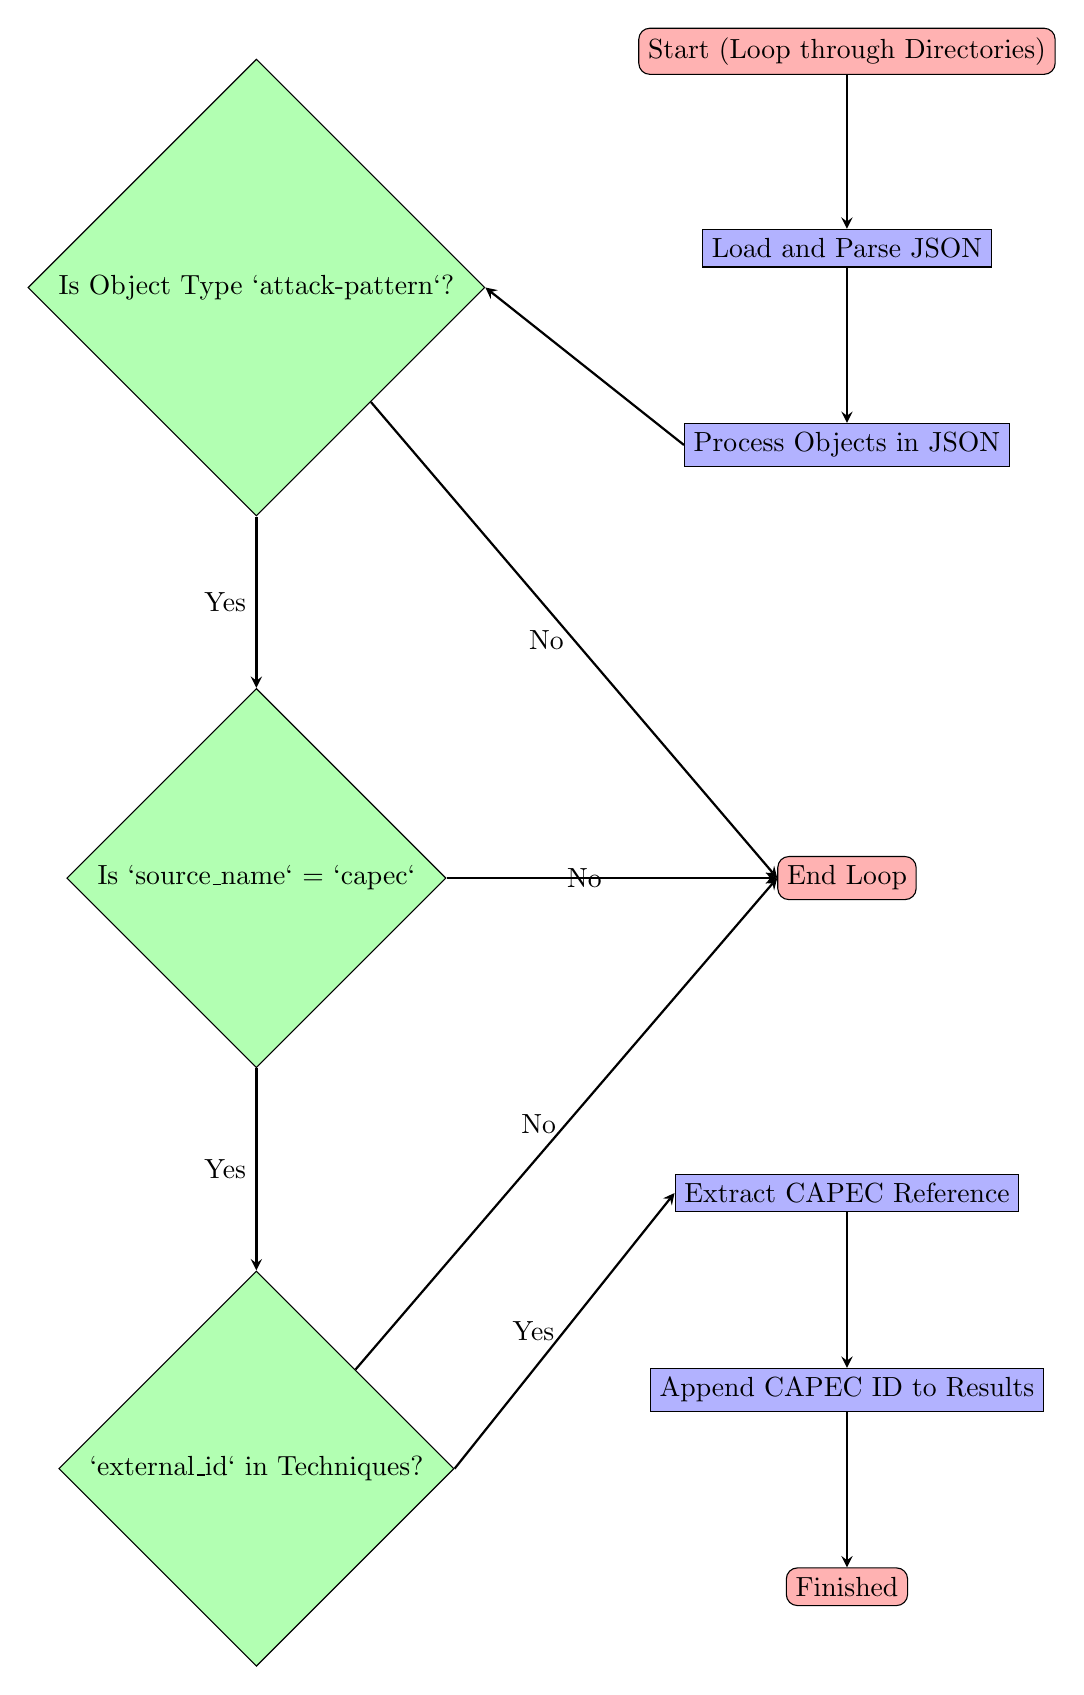
\begin{tikzpicture}[node distance=2.5cm and 3cm]

        % Nodes for processes and start
        \node (start) [startstop] {Start (Loop through Directories)};
        \node (loadJson) [process, below of=start] {Load and Parse JSON};
        \node (processObjects) [process, below of=loadJson] {Process Objects in JSON};
        \node (extractCapec) [process, below of=processObjects, yshift=-7cm] {Extract CAPEC Reference};
        \node (appendCapec) [process, below of=extractCapec] {Append CAPEC ID to Results};

        % Nodes for decisions (aligned left)
        \node (checkType) [decision, left of=start, xshift=-5cm, yshift=-3cm] {Is Object Type `attack-pattern`?};
        \node (checkRef) [decision, below of=checkType, yshift=-5cm] {Is `source\_name` = `capec`};
        \node (checkTechnique) [decision, below of=checkRef, yshift=-5cm] {`external\_id` in Techniques?};

        % Node for Stop and finish
        \node (end) [startstop, right of=checkRef, xshift= +5cm] {End Loop};
        \node (finish) [startstop, below of=appendCapec] {Finished};


        % Arrows from processes to decisions
        \draw [arrow] (processObjects.west) -- (checkType.east);
        \draw [arrow] (start) -- (loadJson);
        \draw [arrow] (loadJson) -- (processObjects);

        % Arrows between decisions
        \draw [arrow] (checkType) -- node[anchor=east] {Yes} (checkRef);
        \draw [arrow] (checkRef) -- node[anchor=east] {Yes} (checkTechnique);

        % Arrows for "No" to End Loop
        \draw [arrow] (checkType.south east) -- node[anchor=east] {No} (end.west);
        \draw [arrow] (checkRef.east) -- node[anchor=east] {No} (end.west);
        \draw [arrow] (checkTechnique.north east) -- node[anchor=east] {No} (end.west);

        % Arrow from last decision to process
        \draw [arrow] (checkTechnique.east) -- node[anchor=east] {Yes} (extractCapec.west);

        % Arrow from processes to the next
        \draw [arrow] (extractCapec) -- (appendCapec);
        \draw [arrow] (appendCapec) -- (finish);

    \end{tikzpicture}
    \caption{Detailansicht der Ablaufs des Mapping MITRE-Technik zu CAPEC.}
    \label{fig:detailed-mapping}
\end{figure}

Wenn alle Mappings über die verbesserte Implementierung gefunden wurden, werden die Ergebnisse mit den Ergebnissen aus der originalen Implementierung zusammengeführt. Dadurch ergibt sich das komplette Mapping von \gls{mitre}-Technik zu \gls{capec}. Für die anderen Schritte des Mappings wurden keine Verbesserungsmöglichkeiten gefunden, daher sind die Funktionen aus dem originalen Quellcode beibehalten worden. Ein Ablaufdiagram dieser Funktionen ist im Anhang \ref{app:flow-acema} dargestellt. \todo{Andere Flow Diagramme wirkklich nötig??}

Aktuell gibt es keine Möglichkeit die \gls{acema} Python Skripte aus dem Dashboard heraus auszuführen, um eine neue Datensammlung oder Datenauswertung zu starten. Die Änderungsrate der Daten ist zudem eher gering. Die \gls{mitre}-Techniken im Dashboard sind quasi statisch, da sie sich an den implementieren Szenarien des Attack-Tools und dem \gls{attack}-Framework in Version \textit{16.1}orientieren. Die Gesamtmenge aller \glspl{capec} umfasst 559 in \gls{capec} Version \textit{3.9}, wobei seit Januar 2023 nur vier neue (+0,7\%) hinzugefügt wurden. Auch die Veränderung im Mapping zwischen \gls{capec} und \gls{cwe} ist gut dokumentiert auf der \gls{capec} Webseite einsehbar. Hier ist eine Veränderung von 59 neu hinzugefügten Mapping in Version \textit{3.9} vor dem Hintergrund der Gesamtmenge auch eine sehr kleine Veränderung. Die Gesamtmenge der \gls{capec}-zu-\gls{cwe}-Mapping lässt sich anhand folgender Daten aus dem Testdatensatz in Anhang \ref{app:mapping-dataset} und den Werten aus \autocite{CAPECNewsEvents} schätzen:
\[
\begin{alignedat}{2}
&\text{Anzahl von } \glspl{capec} \text{ in Testdatensatz} &\quad &= 29 \\
&\text{Anzahl von } \glspl{cwe} \text{ in Testdatensatz} &\quad &= 119 \\
&\text{Durchschnittliche Anzahl von } \frac{\glspl{cwe}}{\gls{capec}} &\quad &= 4{,}1 \\
&\text{Schätzung der Anzahl der Mappings} &\quad &= \text{Gesamtmenge von } \glspl{capec} \times 4{,}1 \\
&&&\thickapprox2300 \\
\end{alignedat}
\]
Zu einem ähnlichen Wert von 1700 bis 2800 kommt auch OpenAI ChatGPT 4o, wobei dort mit Werten von 3 bis 5 für die Anzahl der durchschnittlichen \glspl{cwe} pro \gls{capec} gerechnet wird \autocite{openaichatgpt4oCAPECCWEMapping2024}.

Zu Letzt muss noch das Mapping von \gls{cwe} zu \gls{cve} betrachtet werden. Die Daten dazu stammen aus der \gls{mitre} \gls{cwe} Liste und werden mehrmals jährlich, ungefähr alle vier Monate aktualisiert \autocite{CWEDownloads} \autocite{AIWorkingGroupMeeting_slides20241115_CWEAIWGpdf}.

Das Mapping zwischen \gls{mitre}-Technik und \glspl{cve} ändert sich in Folge dessen nur in geringer Weise. Eine Integration der neuen Daten durch das Ausführen der \gls{acema} Skript und das Kopieren der \verb|json|-Datei in die Dashboard Verzeichnisse \verb|pkg\artifacts| und \verb|pkg\mitre| ist demnach nicht kontinuierlich, aber mit einem Abstand von ungefähr vier Monaten, angepasst an die Änderungsrate der \gls{cwe} Liste, empfehlenswert.


\section{CVSS Integration}
\label{sec:impl-cvssIntegration}
Eine Integration mit dem \gls{cvss} ist eine grundlegende Funktion für jede Anwendung, die eine Bewertung von Schwachstellen vornimmt. Der \gls{cvss} Wert hilft dabei, schnell einen Überblick über den Schweregrad eines potentiellen Angriffs durch Ausnutzung der spezifischen Schwachstelle zubekommen. Aus diesem Grund hatte die Umsetzung von Beginn an eine hohe Priorität. Ursprünglich sollte die Bewertung nur über manuell zugeordnete \glspl{cve} vorgenommen werden, diese Ansatz stellte sich allerdings als mühsam und nicht praktikabel heraus. Über die in Kapitel \ref{sec:impl-anwendungVonAcema} beschriebene Implementierung von \gls{acema} war eine deutlich schnellere und automatisierte Anreicherung von Daten mit \glspl{cve} möglich. Die Visualisierung der \gls{cvss} Werte wurde an zwei Stellen implementiert, die im Folgenden genauer betrachtet werden.

\par Die Visualisierung von einem durchschnittlichen \gls{cvss} für eine \gls{tm4k}-Technik in der Matrix ist einer der Anwendungszwecke, die durch das von \gls{acema} erstellte Mapping möglich gemacht wird. Dabei wird für eine Technik der Durchschnitt aller \gls{cvss} \textit{v2\_score} Werte in den zugeordneten \glspl{cve} gebildet. Wie bereits in Kapitel \ref{limitationen-acema} beschrieben, nutzt \gls{acema} das \gls{cvss} in \textit{Version 2}. Die Metrik \textit{v2\_score} ist dabei ein Wert aus der \textit{Gruppe der Basismetriken} und beschreibt die grundlegenden Merkmale einer Schwachstelle, die im Gegensatz zu Metriken aus der \textit{Zeitlichen Gruppe} und der \textit{Umgebungsgruppe} nicht über die Zeit verändern \autocite{CVSSV2Complete}. Die vollständigen Schritte der Zuordnung sind in Abbildung \ref{fig:mitre_mapping} dargestellt. Zu \~90\% der im Dashboard dargestellten Techniken ist eine \gls{mitre}-Technik zugeordnet  und über \gls{acema} können für diese insgesamt 306 relevante \glspl{cve} gefunden werden. Diese Menge an \glspl{cve} bietet eine ausreichende wissenschaftliche Basis zur Auswertung von \gls{cvss} Daten. 

\par Eine weitere Anwendung findet die Integration mit \gls{cvss} Daten in der Übersichtsseite eines Artefakts. Die dort angezeigten Werte sind auch wieder Durchschnittswerte, die sich aus den \glspl{cve} zusammensetzen, die genau der einen \gls{mitre}-Technik in diesem Artefakt zugeordnet wurden. Der \textit{Average Score} für ein Artefakt unterscheidet sich deshalb vom Wert der in der Matrix für die \gls{tm4k}-Technik angezeigt wird, wenn zwei verschiedene \gls{mitre}-Techniken dieser zugeordnet sind. Das ist in circa 18\% der \gls{tm4k}-Techniken der Fall. \todo{Relevanz??}
Zusätzlich zu diesem generellen Durchschnittswert wird in der Detailansicht ein Wert dargestellt, der die Auswirkung und die Ausnutzbarkeit der zugeordneten \glspl{cve} darstellt. Diese Metriken stammen aus der \textit{Gruppe der Basismetriken} \autocite{CVSSV2Complete}.

\par In beiden Fälle ergänzt eine farbliche Darstellung die numerischen Werte. Die Implementierung im \textit{Go} Quellcode ist in Listing \ref{list:scorecolor} gezeigt. Die Schwellwerte, die ein Spektrum zu einer diskreten Farbe abbilden können hier angepasst werden. Diese Funktion wird dann über die \verb|template.FuncMap| als Funktion definiert, die direkt in einer \verb|.tmpl| Datei genutzt werden kann. \textit{Go Templates} (deutsch: Vorlagen) werden in \textit{Go} genutzt, um datengesteuert HTML-Seiten mit dynamischen Daten aus einer Datenquelle zu befüllen. Die Datenquellen sind in der Implementierung der das Dashboard Objekte oder eine Liste von Objekten vom Datentyp \verb|Tactic|, \verb|Technique| und \verb|Artifact|. Die Möglichkeit, eine Funktion über \verb|template.FuncMap| verfügbar zu machen, erweitert die Standardfunktionen der Vorlagen-Engine und erlaubt es, komplexe logische Operationen oder Formatierungen direkt im Template auszuführen. Dies führt zu einer klaren Trennung von Logik in \textit{.go} und Darstellung in \textit{.tmpl} Dateien \autocite{TemplatePackageText}.

\begin{code}[caption={Implementierung der farblichen Kategorisierung von Schweregraden}]
func ScoreColor(score float64) string {
    switch {
    case score > 7.0:
        return "danger"
    case score > 3.0:
        return "warning"
    case score == 0.0:
        return "secondary"
    default:
        return "success"
    }
}
\end{code}
\label{list:scorecolor}
Die Darstellung von einzelnen GUI-Elementen wird durch die Nutzung von Bootstrap-Komponenten unterstützt. Bootstrap bietet unter anderem vorgefertigte \textit{Badges} (deutsch: Plaketten) an, die genutzt werden um zum Beispiel den \gls{cvss} Wert für eine Technik in der Matrix darzustellen. Die Nutzung von \textit{Badges} ist in Abbildung \ref{fig:cvss-colors}, die zugehörige Zeile des Quellcodes in einer Template-Datei ist in Listing \ref{listing:template-cvss} gezeigt \autocite{contributorsBadges}.

Die Rückgabe der Funktion \verb|ScoreColor| wird im Template direkt als String in die Definition einer \textit{Badge} eingefügt. So lassen sich vorgefertigte Farben anhand von damit assoziierten Adjektiven auswählen. Am Beispiel von Listing \ref{listing:template-cvss} wird erkennbar, dass die Funktion \verb|scorecolor| mit dem Attribut \verb|AvgV2Score| eines Artefakts als Parameter aufgerufen wird, dessen Rückgabe die Klasse des HTML-Elements \verb|span| definiert. Der tatsächliche Wert des Attributes wird dann innerhalb des Elements ausgegeben \autocite{HTMLSpanTag}.

\begin{code}[caption=Aufbau eines HTML Elements zur Darstellung eines CVSS Werts in einer Bootstrap Komponente]
    <span class="badge bg-{{ scoreColor .AvgV2Score }}">{{ .AvgV2Score }}</span>
\end{code}
\label{listing:template-cvss}

\todo{Worüber kann ich hier noch mehr schreiben??}

\section{Visualisierung des Angriffspfads}
\label{sec:impl-visualisierungDesAngriffspfads}